<< EM PROCESSO DE RECONSTRUCAO APOS FEEDBACK DO PROF VANDER>>
<<PROFESSORES, FAVOR CONTINUAR VERIFICACAO A PARTIR DA SECAO 3>>



The task allocation problem solution proposed by \textit{Schwarzrock et al.} in \cite{MAS07} was modeled as a generalized assignment problem (GAP) and the goal is to maximize the total capability of the agents using a probabilistic approach \cite{theraulaz1998response}. 







<<Explain it later in this section>> This capability is measured with the suitability level among the tasks associated and onboard sensors available to perform the activities.




An appropriate combination of swarm intelligence \cite{MOEA07} and a generalized allocation problem (GAP) strategy \cite{ferreira2007swarm} allows to generate an algorithm, based on token transmissions, that the agents perceives in the environment or receives them from a central unity, and does the correct and optimized allocation among them. Algorithm \ref{algo:swarm-gap} shows the pseudo code (from \cite{MAS07}) that implements this combination called swarm-GAP to solve an allocation problem among agents. 

\begin{algorithm}[!ht]
	\SetAlgoLined
	\DontPrintSemicolon
	\SetKwBlock{Loop}{loop}{end loop}
	\SetKwFor{ForAll}{for all}{do}{end for}
	\SetNlSty{text}{}{:}
	\SetNlSkip{0.3em}	
	
	\caption{Pseudo code of the Swarm-GAP (from Schwarzrock et al.) }
	\label{algo:swarm-gap}
	Receive Token\; \label{line:receivetoken}
	Compute available resources $r_i $ \; \label{line:compute_r}
	\ForAll{ available tasks }{ \label{line:forall}
		Compute capability $k_{ij}$\; \label{line:compute_k}
		Compute tendency $T_{\theta_{ij}(st)}$ \;  \label{line:compute_t}
		\If{ roulette() $< T_{\theta_{ij}(st)}$ and $r_i \geq c_j $}{ \label{line:ini_ifalgo1}
			Allocate task $j$ to agent $i$ \; \label{line:aloca_sgap}
			Decrease resource $r_i $\; \label{line:decrease_r} \label{line:fim_ifalgo1}
		}
	}
	Mark agent as visited in the token\; \label{line:marcavisitado}
	\If{there are still available tasks}{ \label{line:ifstillavatask}
		Send the token to a not yet visited agent\; \label{line:envia}
	}
\end{algorithm}

A set of tasks defines a mission that is transmitted to the UAV team by a Central Command. Running the allocation algorithm, each UAV can perform more than one task but each task can be performed by only one agent. The mission transmission is done using a token-based protocol that transmits all information about the tasks and agents association. With this protocol, when a specific UAV chooses a task and allocate it to itself, it sends this information to the next agent of the team. Thus, the next agent will know which tasks are available to be executed.

However, this communication mechanism has some drawbacks <<Which one>> that are listed by the original study \cite{MAS07} and due to these issues, \textit{Schwarzrock et al.}\cite{MAS07} proposed three variations based on swarm-GAP algorithm  as listed bellow:

\begin{itemize}
   \item \textit{Allocation Loop (AL)}: a control list of visited agents is used and the token runs while there is task available. To avoid the infinite loop, the agent registers if it has any resource available to perform a new task before resend the token. Only the agent with free resources will receive the token;
   \item \textit{Sorting and Allocation Loop (SAL)}: sorts the list of tasks based on the tendency($\textrm{T}_{\theta_{ij}}$) of execution by the UAV. This prevents the first agent, during the token exchange, from being assigned all tasks, not considering others UAVs more suitable to perform some of these tasks and producing better results. 
   
   
   agent from roundThis avoids the first agent gets all tasks instead of them that are more suitable and produces better results;
   \item \textit{Limit and Allocation Loop (LAL)}: increases the SAL behavior and defines a task selection limit per UAV in each round to avoid to adopt a greedy strategy and leaves idle agents;
\end{itemize}

The team agents have a mission to be performed, and it is composed by one or more tasks. To perform the mission, the team has a limited time defined in ticks. All experiments executed by this work and the original one, are using the same time slice of 300 ticks. The displacement and task execution have a time consumption and the total has to be inside this limit.

An important attribute of the algorithms handled, that represents the agent will to perform a task is called $stimulus (st)$. It balances the weight among the distance to the task and sensor quality. Previous studies, as in \cite{ferreira2007swarm} and  \cite{MAS07}, showed and justified that the more suitable value in most situations is $0.6$. This $stimulus$ contributes to the calculation of the agent tendency  (Equation \ref{eq:tendencia}). And the agent threshold $\theta$ to perform a task is shown in Equation \ref{eq:limiar}. Higher $stimulus$ indicates that less specialized agents will perform the tasks. In another hand, if $stimulus$ is lower the task performing will be done by more specialized agent.\cite{bonabeau1999swarm}.

\begin{equation} \label{eq:tendencia}
	\textrm{T}_{\theta_{ij}}(st_j) = \frac{st_{j}^2}{st_{j}^2 + \theta_{ij}^2}
\end{equation}

\begin{equation} \label{eq:limiar}
	\theta_{ij} = 1 - k_{ij}
\end{equation}

Where agent $i$ has a specific capability $k_{ij}$ (see Equation \ref{eq:capability}) to perform each task $j$, and $J$ is the set of available tasks, $d(i,j)$ is the Euclidean distance between the UAV and the task, $Q(i,j)$ is the UAV's quality to perform the task and $\alpha \in [0,1]$  is the weight given to the distance and quality factors. 

\begin{equation} \label{eq:capability}
\begin{split}
k_{ij} = \frac{\max_{g \in J} \{d(i,g)\} - d(i,j)}{\max_{g \in J} \{d(i,g)\}} \times \alpha + \\
(1 - \frac{\max_{g \in J} \{Q(i,g)\} - Q(i,j)}{\max_{g \in J} \{Q(i,g)\}}) \times (1-\alpha)
\end{split}
\end{equation}


To perform experiments based on a previous work, repeating procedures or changing parameters, it is needed to analyze the reproducible research (RR) level of the study. According to Madeyski and Kitchenham in \cite{exp02} the RR is referenced to the level of how the experiment can be reproduced from the original data and information by others researchers. With a reproduction, the results obtained by the primary work can be validated and the information published completeness can be checked. Besides there is a significant difference between the concepts of RR and replication \cite{exp02} \cite{exp03}.

Elements of impact on experiment reproducibility level can be seen in Figure \ref{grafico:elements} adapted from González et al. in \cite{exp05}. Each of these elements represents an object that can be reused in a new research. The data source is the repository or object that has all data of experiment interest. Raw Dataset represents all data retrieved, normally using a software tool, from the data source. All data extracted from the Dataset represents a processed Dataset and, after an analysis, these information generates a result Dataset.

\begin{figure}[h]
	\begin{center}
		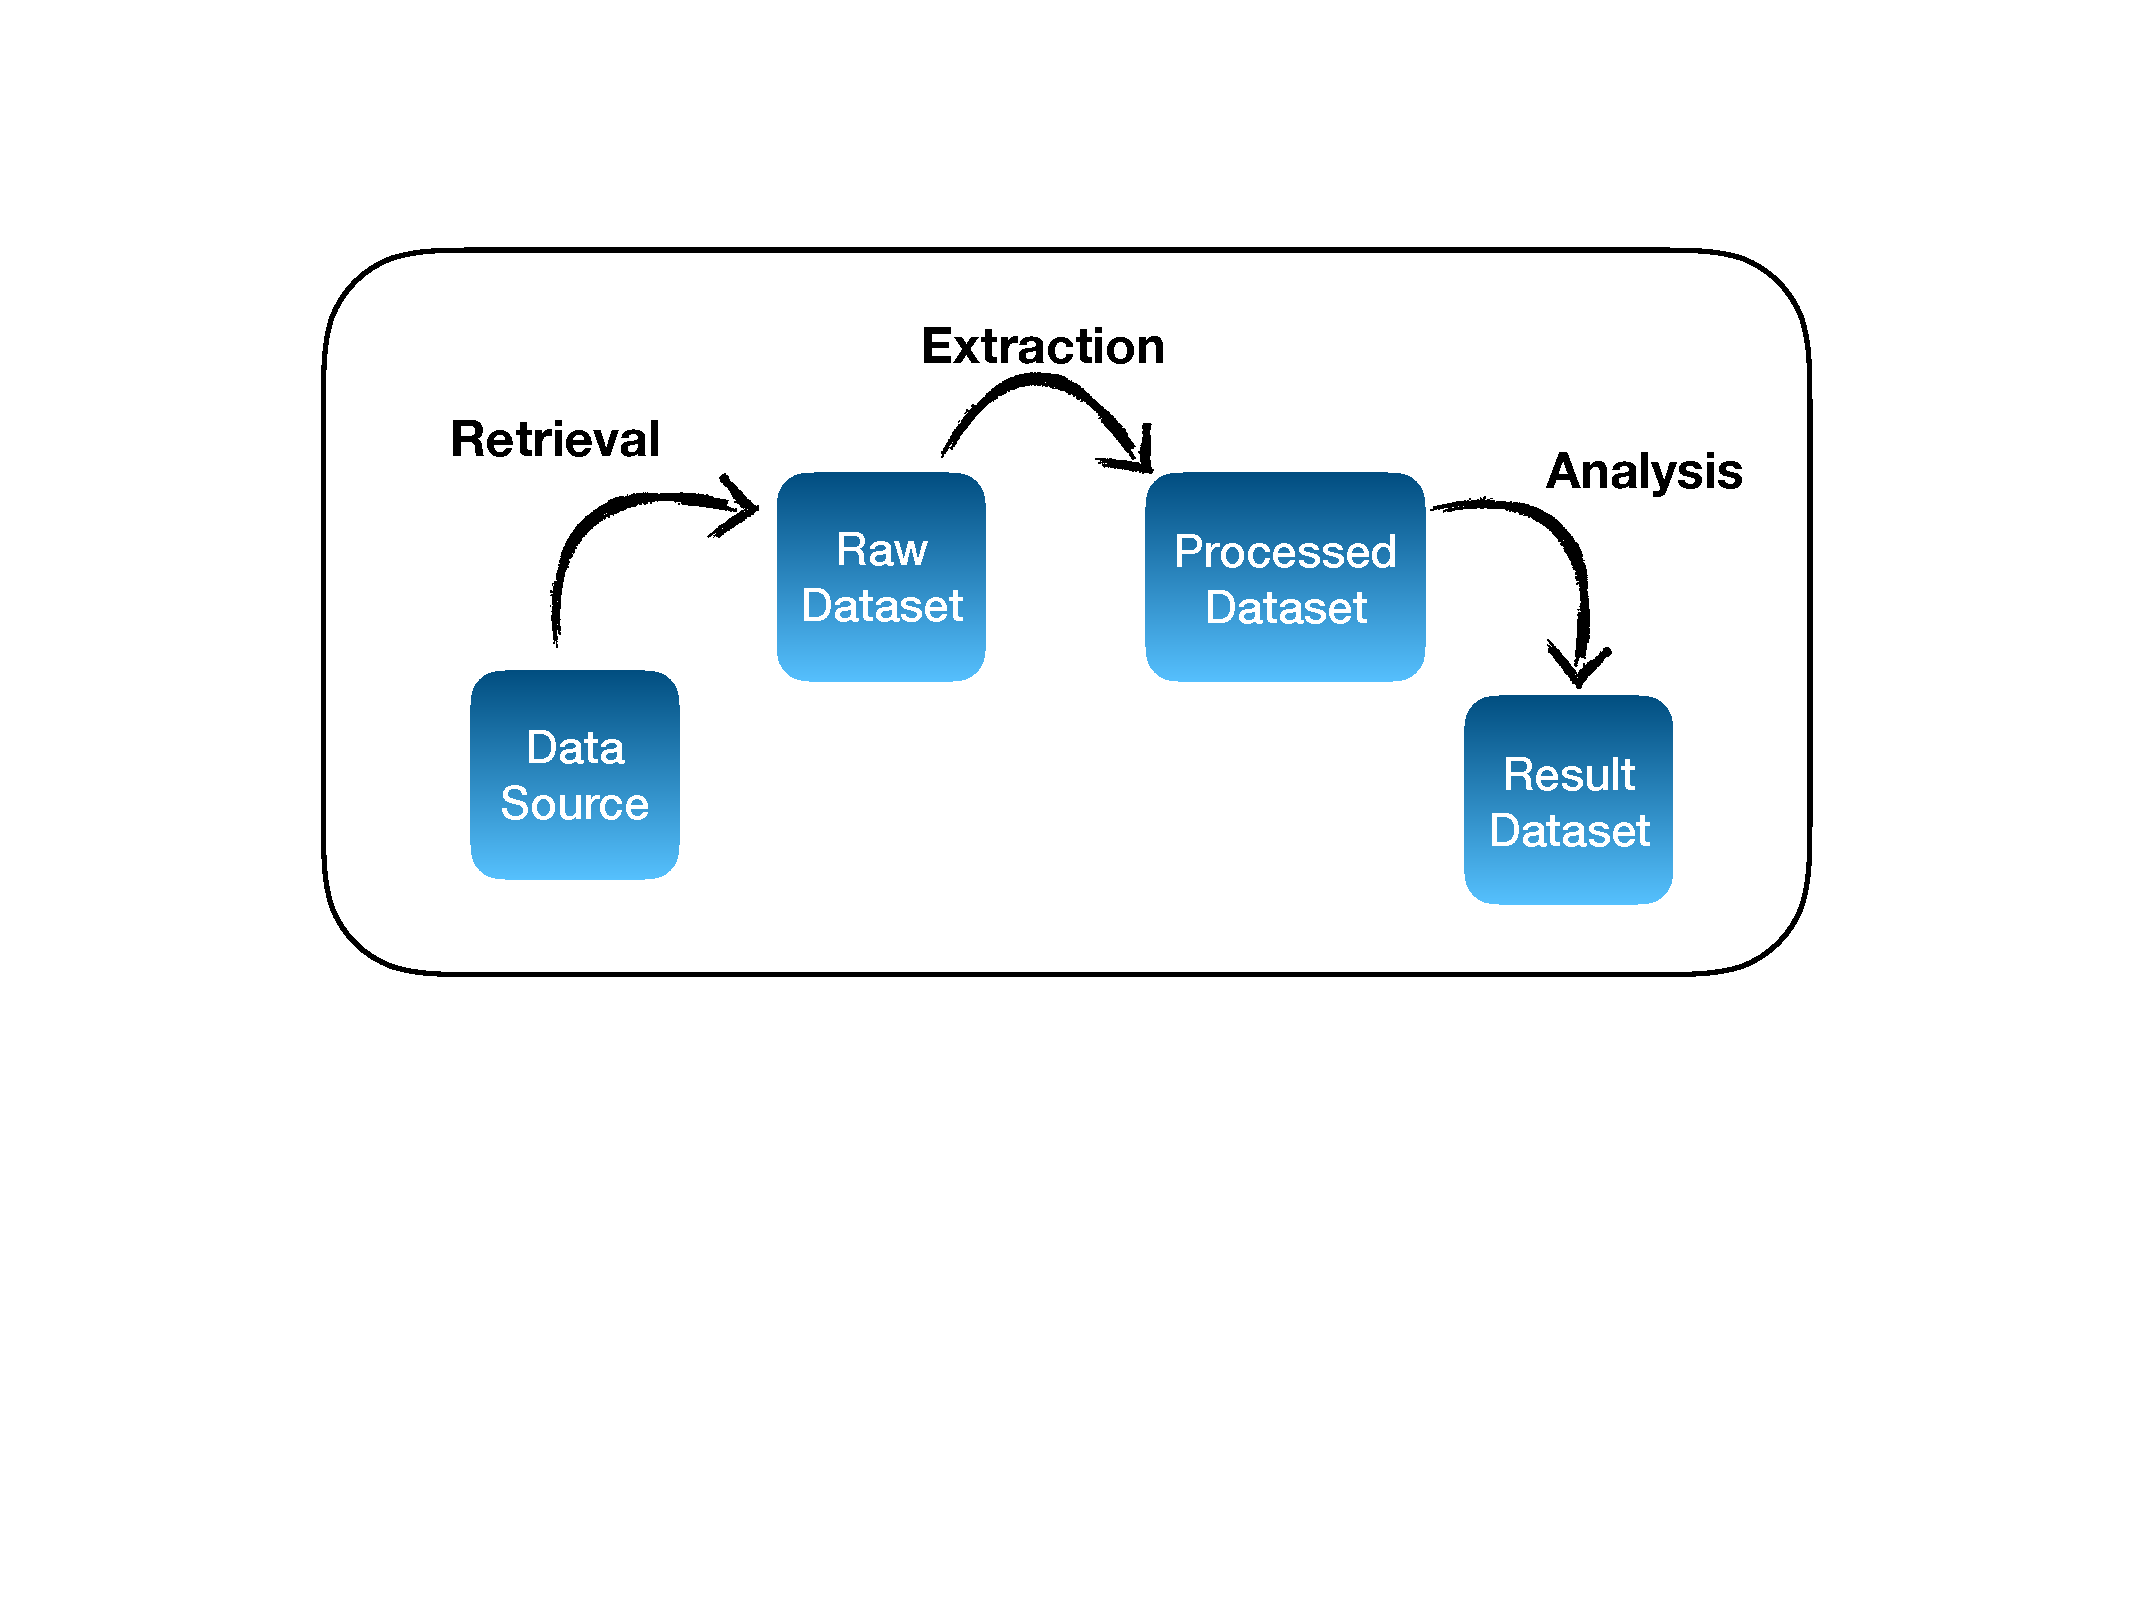
\includegraphics[scale=.35]{diagrama01.pdf}
		\caption{Elements of interest for reproducibility (Adapted from González et al.)}
		\label{grafico:elements}
	\end{center}
\end{figure}

This model was proposed to represent the data retrieving and processing in a empirical software engineer study \cite{exp05}. The main idea is to identify elements that can be reused during the experiment replication and to measure its reproducibility.

Replication in its all levels and types presented by González et al. in \cite{exp03} can creates different contexts from the original study or experiment. Variables, conditions and controls can be change to analyze the effects and impacts over the results. In empirical software engineer studies is common to apply replication in experiments to analyze the system behaviour under some conditions changes.

A specific case of replication called exact replication \cite{exp04} follows all procedures of an experiment as closely as possible to determine how the results obtained will be equals to the original experiment. In this case, the concepts reproduction and replication become the synonyms. The opposite situation occurs with the conceptual replication, where a different experimental procedures are used to prove hypotheses and to answer the research questions. 
